\paragraph{Gestione questionari}

\subparagraph{Gestione iscrizionil questionario}
\label{Recupero risultati del questionario}
\begin{figure}[ht]
	\centering
	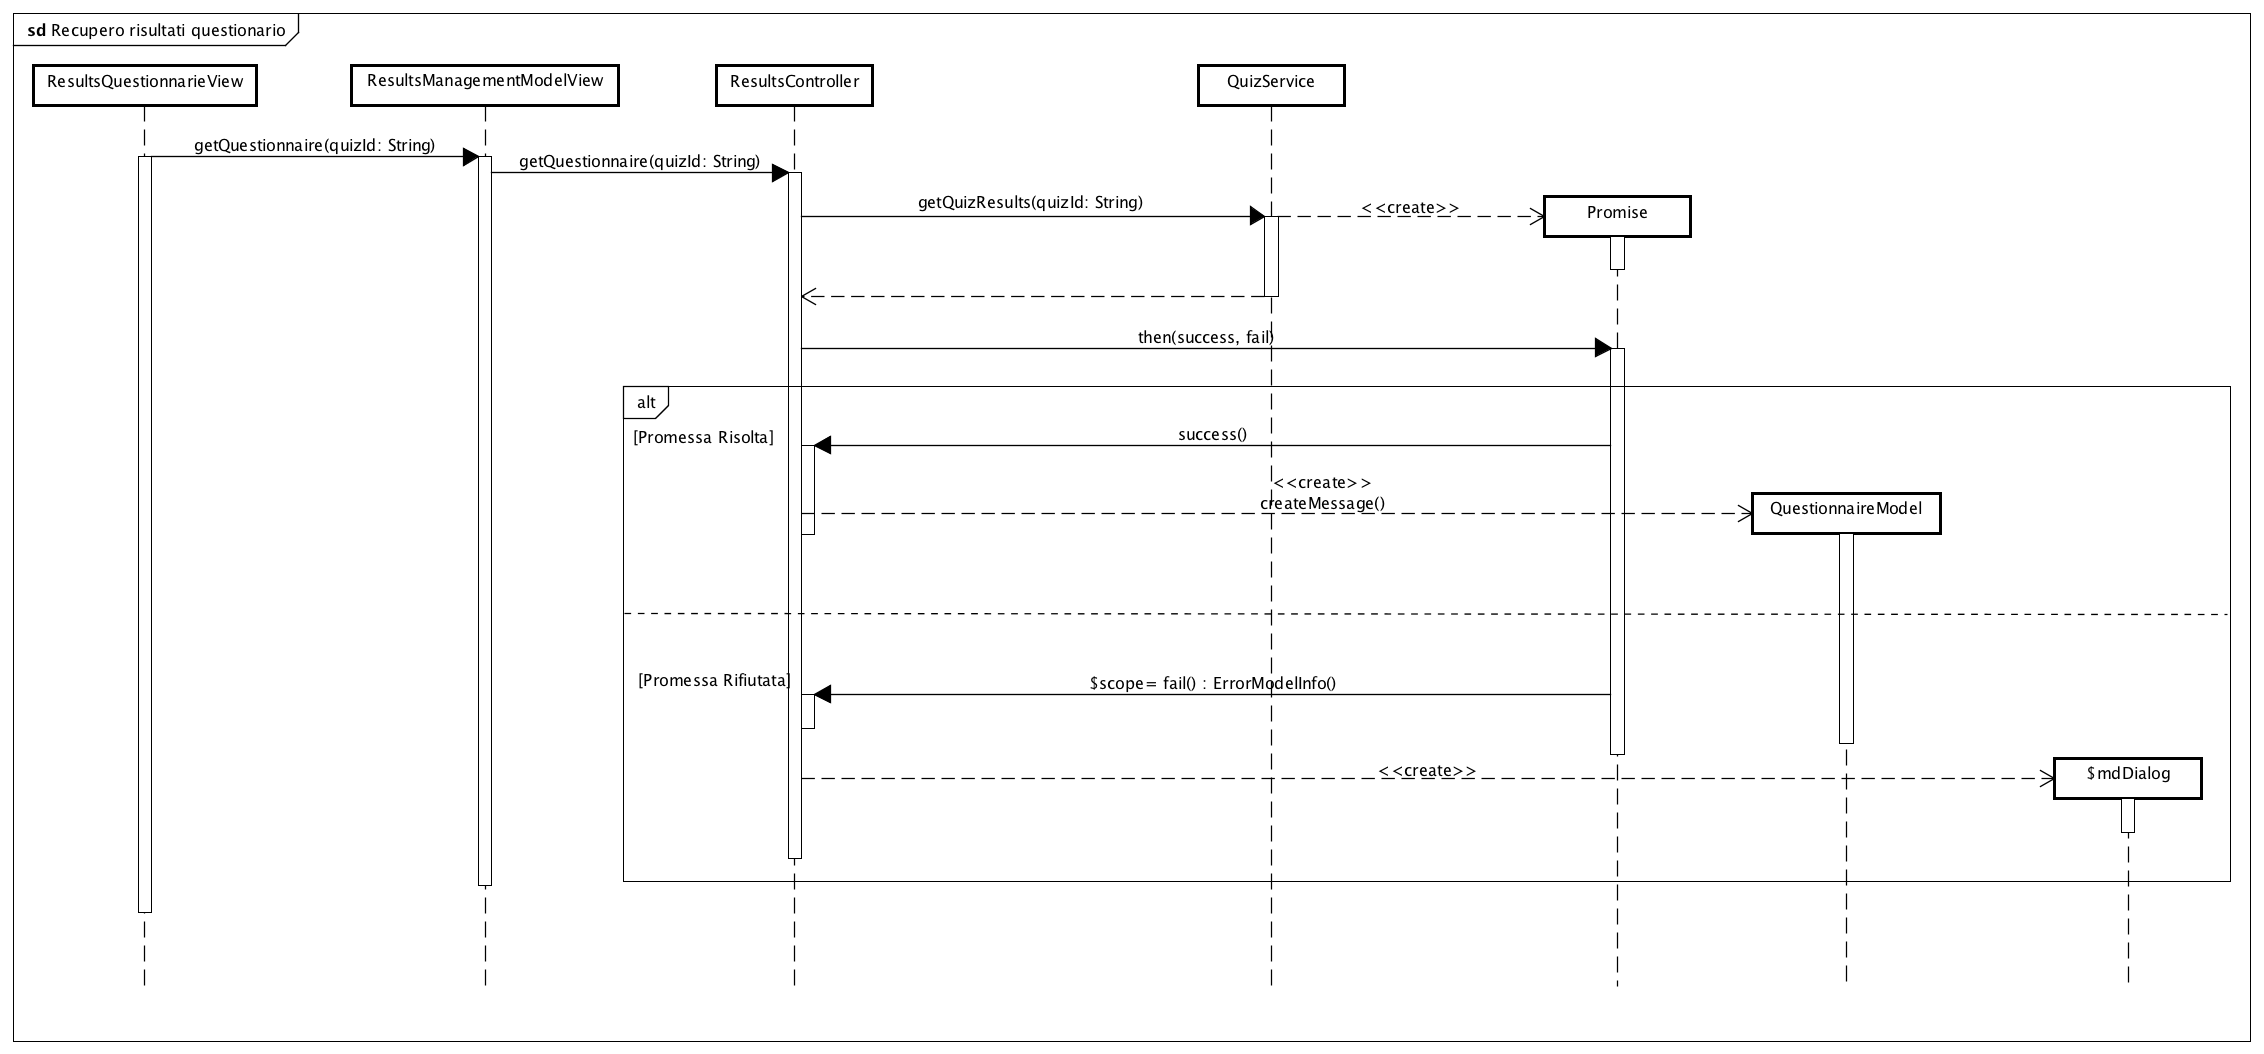
\includegraphics[scale=0.25,keepaspectratio]{UML/DiagrammiDiSequenza/Front-end/ResultsManagement.png}
	\caption{Recupero risultati del questionario}
\end{figure} \FloatBarrier
 
Al momento del caricamento della pagina viene richiamato il metodo del controller che, a sua volta, richiama il metodo del service per ottenere i risultati complessivi del questionario. Se la promessa ritornata dal service viene accettata allora verranno ricevuti i dati, altrimenti verrà restituito un oggetto contenente l'errore.


\paragraph{Recupero utenti del questionario}
\label{Recupero utenti del questionario}
\begin{figure}[ht]
	\centering
	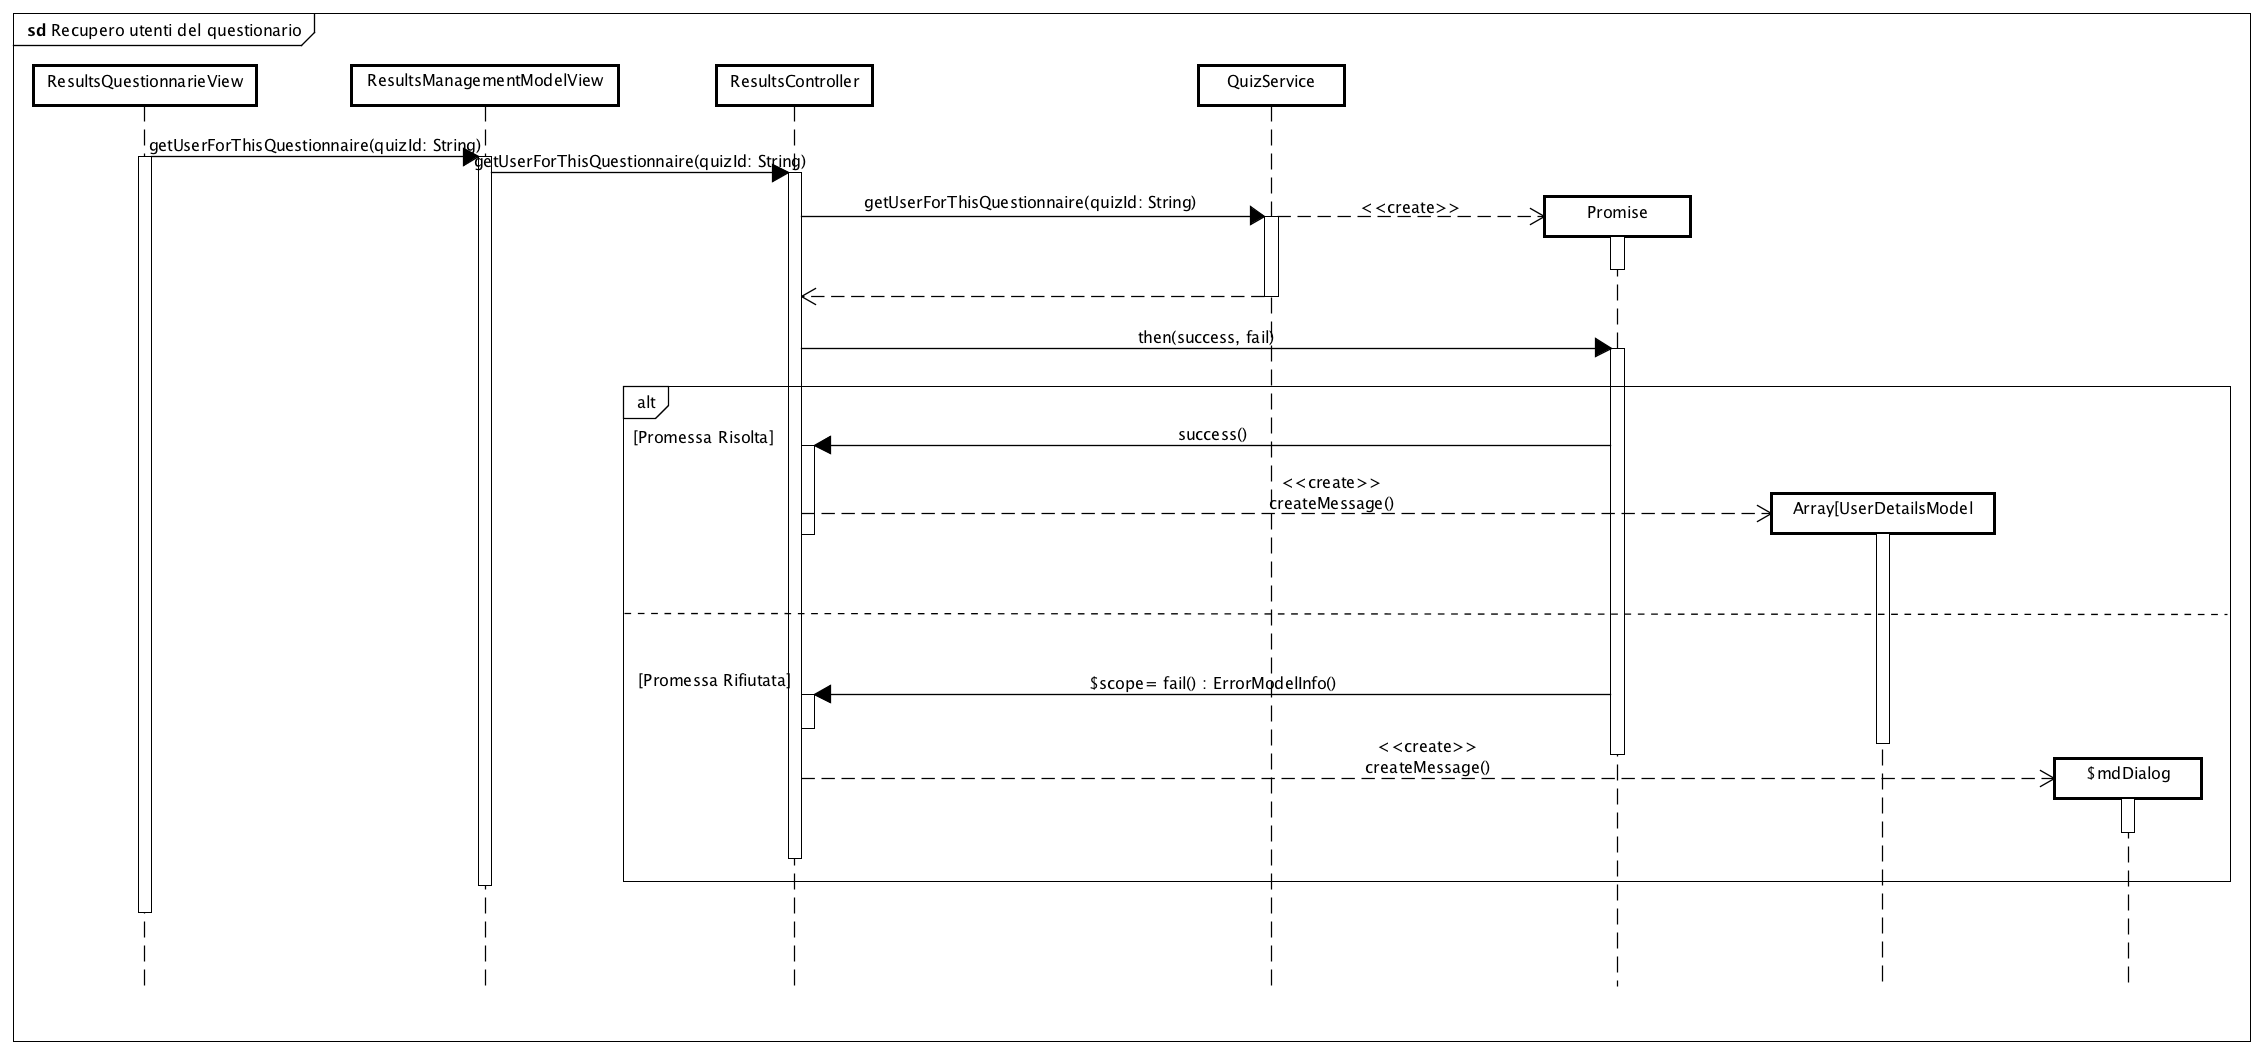
\includegraphics[scale=0.25,keepaspectratio]{UML/DiagrammiDiSequenza/Front-end/GetUsersForQuestionnaire.png}
	\caption{Recupero singoli utenti del questionario}
\end{figure} \FloatBarrier

Al momento del caricamento della pagina viene richiamato il metodo del controller che, a sua volta, richiama il metodo del service per ottenere i singoli utenti del questionario. Se la promessa ritornata dal service viene accettata allora verranno ricevuti i dati, altrimenti verrà restituito un oggetto contenente l'errore.

